\documentclass[11pt]{article}
\usepackage[margin=1in]{geometry}
\usepackage{amsmath,amssymb}
\DeclareMathSizes{10}{10}{8}{6}
\usepackage{graphicx}
\usepackage{booktabs}
\usepackage{xcolor}
\usepackage[colorlinks=true,linkcolor=blue!55!black,citecolor=blue!45!black,urlcolor=blue!55!black]{hyperref}
\usepackage{natbib}
\usepackage{titlesec}
\titlespacing*{\section}{0pt}{1.1em}{0.5em}
\titlespacing*{\subsection}{0pt}{0.8em}{0.3em}

\newcommand{\Sz}{\mathcal{S}_0}
\newcommand{\Zz}{\mathcal{Z}_0}
\newcommand{\Rd}{\mathcal{R}_d}

\title{\vspace{-2em}\textbf{Epigenetic Language Models: Lifelong Learning by\\ Intercalating Knowledge into Structural Zeros}\\[0.3em]\large Free-Slot Adaptation on a real 8B ternary MoE}
\author{Parallax / Chutes.ai}
\date{\today}

\begin{document}
\maketitle
\vspace{-1.5em}

\begin{center}
\fbox{\parbox{0.93\textwidth}{\small\textbf{AI-assisted draft.} Generated with AI assistance and revised through repeated
adversarial review; the experiments were run and checked by the authors. The synthetic sections are a
\textbf{dense fp32 mechanism study}; the real-model section evaluates ternary patches on a real 8B
ternary MoE on a 40-fact task (single seed). The pre-registered multi-session epigenesis experiment is
in progress; the personal-model use case (\S\ref{sec:direction}) remains an \emph{untested proposal}.
Code: \texttt{github.com/chutesai/epigenesis}.}}
\end{center}

\begin{abstract}
We study Free-Slot Adaptation (FSA) through a dense fp32 synthetic mechanism assay and a real
8B ternary mixture-of-experts model. FSA freezes the base and writes acquired knowledge into structural
zeros; removing the patch restores the original model exactly. On a 40-fact task, ternary Bop recalls all
80 held-out test items from 812,420 filled slots (a 0.9 MB patch counting positions), with bit-exact
revoke, at +0.027 nats/token general-text damage; regularized LoRA recalls 78/80 with no measurable
damage. This two-item recall difference on one seed is not a significant win: ternary FSA offers a
smaller patch that preserves the packed format, while LoRA with a local penalty has lower damage.
In the synthetic fp32 assay, tuned LoRA remains both more capable and more storage-efficient; masked
retention is exact by construction, and the always-on soft variant degrades with load. All reported
experiments are single-seed. Multi-session acquisition of concepts, the intended personal-model
application, remains untested in a pre-registered experiment now in progress.
\end{abstract}

\section{Introduction}
Adding knowledge to a trained model usually means adding parameters---a LoRA adapter \citep{lora}, an extra
expert, or a full fine-tune that risks forgetting. We ask a narrower question: an extreme-quantized model
has already paid for a pool of weight slots held at zero; can those zeros double as a place to put new
knowledge?

\textbf{Free-Slot Adaptation (FSA).} Store a model in format $\Phi$ (here \texttt{pair8}: ternary weights,
at most two of every four aligned pairs non-zero). Let $\Sz$ be the non-zero support and $\Zz$ the zero
reserve. To learn a new domain $d$: freeze $\Sz$ and shared parameters, train a disjoint slice
$\Rd \subseteq \Zz$, and store a mask $M_d$. At inference the base uses $\Sz$; domain $d$ uses
$\Sz \cup \Rd$. The mechanism is \citet{packnet}'s; the only new element is that the free weights come from
the compression format rather than a pruning pass.

\textbf{What we claim.} The synthetic assay characterizes exact masked preservation, bounded
memorization, and the cost of a dense fp32 reserve. The real-model experiment (\S\ref{sec:real}) shows
that a legal ternary reserve carries facts and revokes exactly. Bop matches, perhaps slightly exceeds,
LoRA's recall on this single-seed task, from a much smaller patch, but at measurable general-text damage;
regularized LoRA remains the lower-damage method. We do not claim an overall advantage over LoRA or
validated multi-session learning.

\textbf{Contributions.} (1) Quantization zeros as a continual-learning reserve, with accounting for
positions, values, scales, and inference format. (2) A synthetic mechanism study: exact masked retention,
a measured reserve maximum, a degrading soft variant, and an indicative, uncontrolled fp32 LoRA
comparison that favors LoRA. (3) Real 8B results: legal ternary patches, latent-free and learn-then-prune
writers, a routing-related KL floor, and a recall--damage--storage comparison. (4) A revocable-patch
contract and a pre-registered, still untested multi-session concept experiment (\S\ref{sec:direction}).

\section{Background and related work}
\textbf{Mask-based continual learning.} PackNet \citep{packnet} freezes kept weights and trains freed ones,
recovering a task by its mask; Piggyback \citep{piggyback} \emph{learns masks over fixed weights} (it does
not refill zeros); HAT \citep{hat} uses hard task-attention and reports \emph{reduced}, not zero,
forgetting; Supermasks \citep{supermasks} make the mask itself the trainable object; Progressive Networks
\citep{progressivenn} add and could drop columns. FSA is PackNet with the free support supplied by the
quantization format. \textbf{Quantized continual learning.} Ada-QPackNet \citep{adaqpacknet} and
TinySubNets \citep{tinysubnets} already combine PackNet-style capacity reuse with quantization; SPDF
\citep{spdf} reopens zeroed pretrained weights for dense fine-tuning. These sharply narrow our novelty; our
distinct element is a reserve \emph{pre-addressed by the deployed format} and composed by union.
\textbf{Parameter-efficient and continual adapters.} LoRA \citep{lora}, QLoRA \citep{qlora}, QA-LoRA
\citep{qalora}; \citet{loralearnsless} find LoRA learns and forgets less than full fine-tuning (a possible
rank explanation, not a theorem); O-LoRA \citep{olora} does continual learning in orthogonal LoRA
subspaces. \textbf{Sparse / composable adaptation.} Diff pruning \citep{diffpruning} and composable sparse
fine-tuning \citep{composablesft}; union of \emph{disjoint} sparse supports is the easy case of the latter.
\textbf{Editing, memory, unlearning.} MEMIT \citep{memit} edits facts in place and can override; FSA adds paths that can
suppress or correct outputs while enabled but cannot edit a base weight; GRACE \citep{grace} and WISE \citep{wise} keep deletable, routed side-memory for sequential edits
while freezing the base; SISA \citep{sisa} is exact unlearning by shard isolation; TOFU \citep{tofu}
benchmarks fictitious-fact forgetting. \textbf{Personalization and retrieval.} OPPU \citep{oppu} attaches a
per-user PEFT module (removed by user identity, not per record); LaMP \citep{lamp} is a personalization
benchmark with retrieval baselines; RAG \citep{rag} and kNN-LM \citep{knnlm} store facts externally and
delete them by dropping a record---the baseline any ``delete a fact'' claim must beat.
\textbf{Low-bit models.} BitNet b1.58 \citep{bitnet158,bitnet2b4t} and LittleBit \citep{littlebit}; our
assay methodology follows knowledge-capacity scaling \citep{knowcap}. Bop \citep{bop} optimizes binary
weights without latent real weights; we extend its gradient-memory rule to ternary birth and death
(\S\ref{sec:writers}).

\section{Method}
\subsection{Format and reserve}
In \texttt{pair8}, weights form aligned blocks of eight (four pairs); each weight is ternary times a scale,
and at most two pairs per block are non-zero. A block thus has $417$ reachable states
($1 + 4\!\cdot\!8 + \binom{4}{2}8^2$), i.e. $\log_2 417/8 \approx 1.088$ bits/weight asymptotically
($1.125$ at a fixed $9$ bits/block), and is $\ge 50\%$ zero \emph{by construction} (ternary alone
guarantees no such fraction). \textbf{Writable reserve.} Zeros inside already-active pairs can be filled while preserving pair
occupancy and the codebook. At two active pairs, opening a third pair is illegal, but filling a zero
member of an active pair is legal. Thus the writable in-codebook reserve is a subset of the full zero
support, not necessarily empty in a full-occupancy block. Opening additional pairs requires spare pair
occupancy or a separate patch outside the codebook. Filled positions and signs must still be stored
for revocation; the joint rate of 1.088 bits/weight is not the marginal price of a filled slot.

\subsection{Adaptation and the soft variant}
\textbf{Hard FSA, domain $d$:} freeze $W[\Sz]$, all shared parameters, and---crucially for the real
format---the discrete pair occupancy and the per-row scales; train only $W[\Rd]$ ($\Rd \cap \Sz = \varnothing$)
with the base live; store $M_d$. Inference: base $\to \Sz$; domain $\to \Sz\cup\Rd$ (needs a task ID).
\textbf{Soft FSA} removes the task ID: freeze the base, train the reserve with a KL penalty keeping
base-input outputs unchanged, and run unmasked. This is Learning-without-Forgetting \citep{lwf} on a frozen
disjoint support, with full base-input replay---a substantial rehearsal resource we note explicitly.

\subsection{Honest accounting}
FSA adds \textbf{zero new logical parameters}: the element count is unchanged. The real ternary
experiment fills only zeros inside active pairs, so a merged patch uses the same packed tensors and
adds no tensors or inference compute. This claim depends on preserving pair occupancy and the serving
format; opening new pairs or using a separate patch can add work. The packed serving path was not
benchmarked (\S\ref{sec:real}). Storage is not free: revocation needs positions and signs in a stored
diff, or the original pack. Learned scales add storage too. A full per-domain mask would cost one bit
per weight; sparse position coding avoids that cost for sparse patches. Frozen row scales constrain
each ternary slot to $\{-\alpha,0,+\alpha\}$, a capacity restriction. Actual position-inclusive patch
sizes are reported in \S\ref{sec:real}; hypothetical trit-only accounting is insufficient.

\section{Theory}
\textbf{Base invariance (by construction, narrow).} Restrict the forward to $M_0$. If adaptation changes
only $W[\Rd]$ with $\Rd\cap\Sz=\varnothing$ and freezes all shared state, the masked base output is
unchanged---an invariance of freezing, which is why measured ``retention $=1.000$'' is a unit test that the
mask was applied (it would hold even if the reserve learned nothing). \emph{Three subtleties:} (i) it is the
\emph{masked} base; with the reserve enabled, the base behavior is not preserved (we measure strongly
negative unmasked retention). (ii) In the real \texttt{pair8} format the decoded weight is
$\alpha\cdot\text{trit}$ and a quantizer that recomputes pair occupancy or scales could change the base; invariance
requires freezing base support, occupancy, and scales, as in \S\ref{sec:real}. (iii) The soft variant is outside this argument entirely.

\textbf{Reserve capacity is accounting, not a law.} We do not vary $\rho$ or the per-slot cost, so the curve
is a memorization curve, not a test of a capacity expression. We therefore report
$K_{\text{reserve}} \approx \kappa_{\text{adapt}}\,B_{\text{patch}}$ with $B_{\text{patch}}$ the measured patch
\emph{bits} and $\kappa_{\text{adapt}}$ an \emph{observed} knowledge-bits-per-stored-bit efficiency
conditional on base, support, scales, and training budget---and note it has no term for the interference
decline we plot.

\section{Experiments}
\label{sec:synthetic}
Synthetic knowledge-capacity assay: disjoint random fact sets $A\to B$ (key$\to$label, $V{=}1024$, so each
fact is $10$ bits of arbitrary lookup), $K = N\log_2 V - \sum\text{CE}/\ln 2$. A $917$k-parameter MLP
($\rho{=}0.5$) is loaded with 128k base facts (base recall only $0.744$---``saturated'' is relative), then
adapted. \textbf{The reserve is a dense fp32 mask}: this is why everything here is a mechanism
demonstration. Single seed; LoRA uses a fixed scale $2.0$ (not the standard $\alpha/r$ of \citet{lora}) with
its learning rate tuned down per load to compensate; it also uses AdamW \citep{adamw} weight decay $0.01$ (vs FSA's $0$) and sees a
dense base (recall $\approx\!0.64$) while FSA sees a $50\%$-masked base (recall $0.744$)---so the comparison
is indicative, not controlled.

\begin{figure}[t]\centering
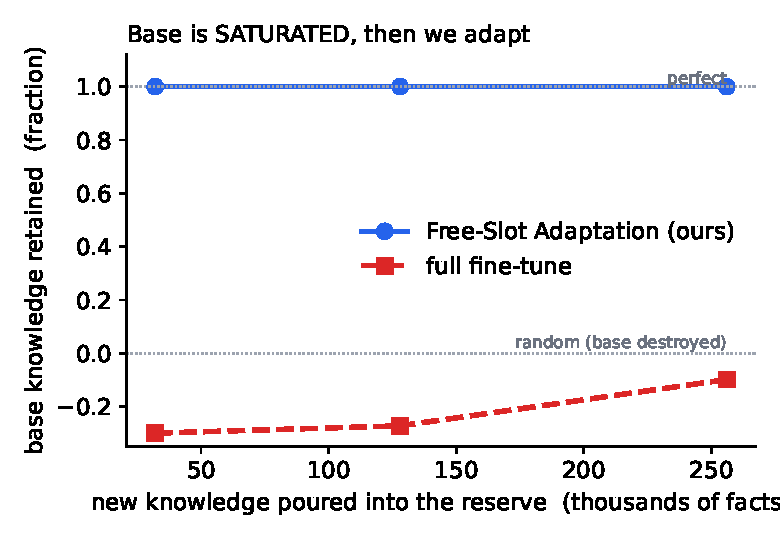
\includegraphics[width=0.48\textwidth]{../figures/fig1_retention.pdf}\hfill
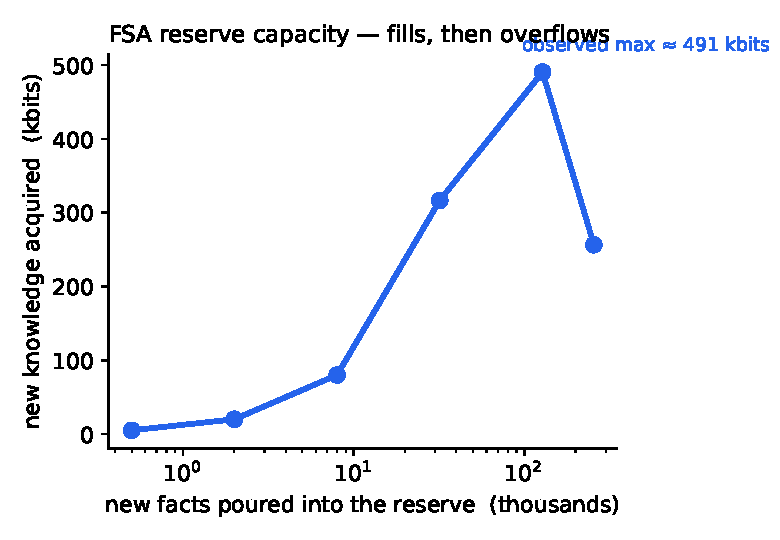
\includegraphics[width=0.48\textwidth]{../figures/fig2_reserve.pdf}
\caption{\textbf{Left:} masked base retention stays $1.000$ (by construction) while full fine-tuning
destroys the base. \textbf{Right:} the reserve memorizes up to $\approx 490.6$ kbits, then \emph{declines}
to $256.5$ kbits at $256$k facts---a maximum under this training budget (fewer exposures per fact as the
count grows can contribute), not a proven intrinsic ceiling.}
\label{fig:core}
\end{figure}

\begin{figure}[t]\centering
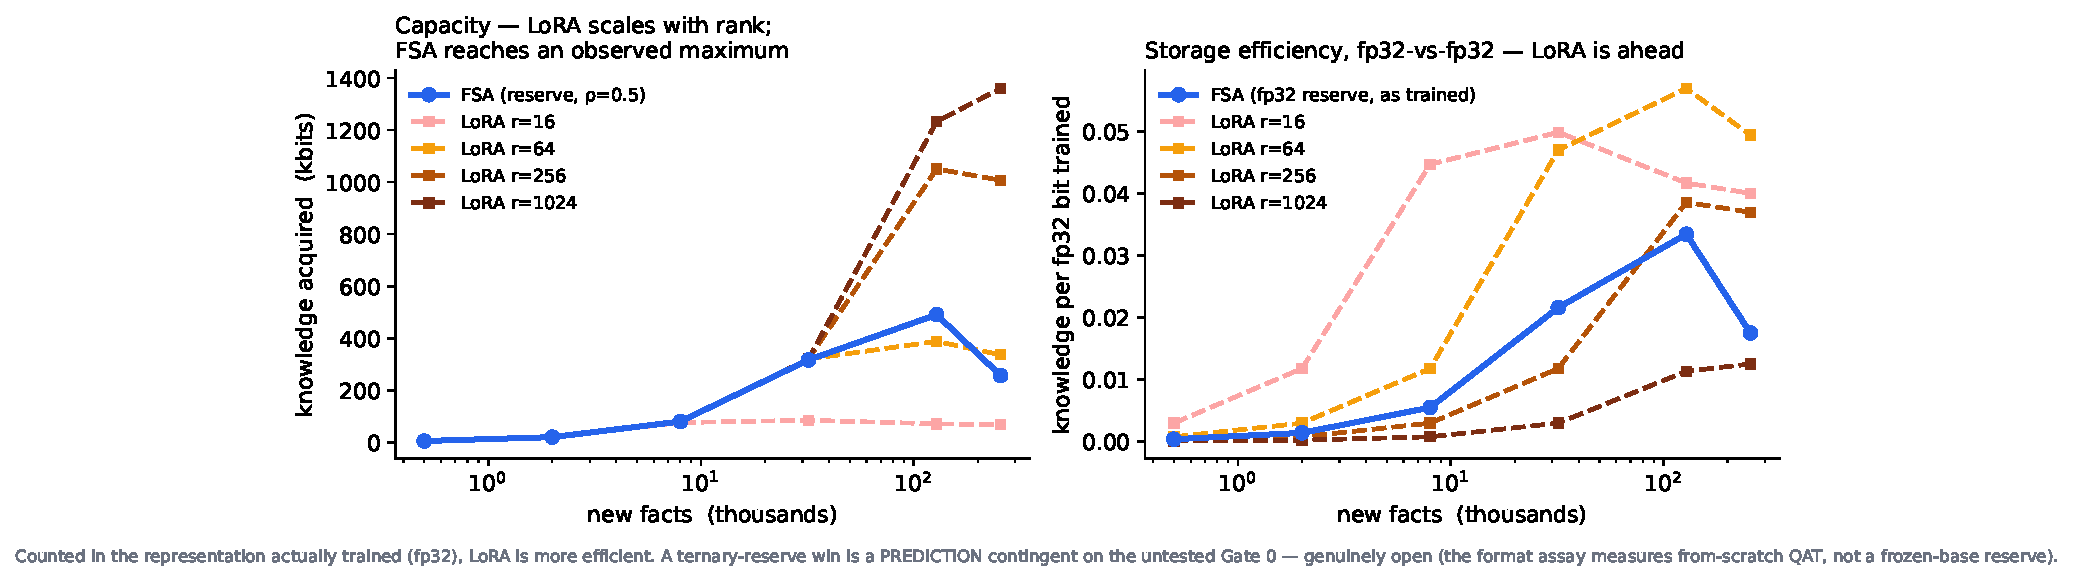
\includegraphics[width=0.95\textwidth]{../figures/fig3_vs_lora.pdf}
\caption{\textbf{FSA vs.\ tuned LoRA.} Left: LoRA's capacity scales with rank and \emph{exceeds} FSA's
reserve maximum at $r\ge 256$. Right: counted in the representation actually trained (fp32), LoRA is
\emph{more} storage-efficient ($\kappa\!\approx\!0.057$ at $r{=}64$ vs FSA $\approx\!0.033$). These are dense fp32 mechanism results; the position-inclusive ternary
patch comparison on a real model is separate (\S\ref{sec:real}).}
\label{fig:lora}
\end{figure}

\textbf{Retention and reserve (Fig.~\ref{fig:core}).} Masked retention is exactly $1.000$; full fine-tuning
goes below random. The reserve fills to $490.6$ kbits and then declines.

\textbf{LoRA (Fig.~\ref{fig:lora}).} With its learning rate tuned, LoRA learns facts well and at $r\ge256$ acquires
\emph{more} than FSA's maximum; counted honestly in fp32 it is also \emph{more} storage-efficient. The smaller ternary patches measured in \S\ref{sec:real} do not change this
fp32 result. Dividing fp32 knowledge by hypothetical trit storage would not be a valid comparison.

\textbf{Soft variant (Fig.~\ref{fig:soft}).} Run unmasked, retention \emph{degrades} with load
($0.98 \to 0.78$ at $8$k facts $\to 0.12$ at $32$k), bought with full base-input replay. We describe this as
degradation, not ``graceful'' suitability. The $\lambda$ weight is a plain retention/acquisition dial.

\begin{figure}[t]\centering
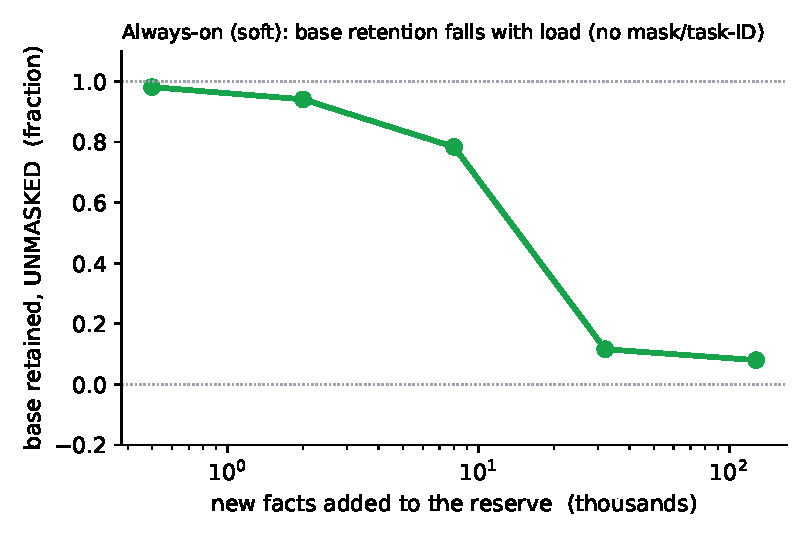
\includegraphics[width=0.52\textwidth]{../figures/fig4_soft.pdf}
\caption{The mask-free soft variant degrades with load (with full base-input replay). It has no addressable
slice to delete.}
\label{fig:soft}
\end{figure}

\section{Real-model results (lambda 8B)}
\label{sec:real}
\begingroup\small
\textbf{Model and protocol.} Lambda is an 8B-parameter ternary MoE with 128 routed experts per MoE
layer, 12 active per token, model width 1152, and a recurrent sequence-mixing state between layers.
Each routed expert has a $2304\!\times\!384$ up projection, squared ReLU, and a
$384\!\times\!2304$ down projection, stored as \texttt{pair8} trits times frozen per-row scales.
We patch layers 14--15, all 128 experts, both projections: a broad footprint with 66,807,179 free slots
inside already-active pairs. Base support, scales, pair occupancy, router, and all other parameters
remain frozen. Ternary births take value $\pm\alpha$ for row scale $\alpha$. The fp4 variant uses an
E2M1 four-bit float grid times $\alpha$, with step $0.25\alpha$ and cap $1.5\alpha$; it leaves the
ternary codebook. Evaluation decodes experts to bf16. Legal ternary patches could use the same packed
kernel, but that serving path was not benchmarked.

The task has 40 synthetic facts about a fictional person (favorite cheese, boat's name, house number).
Training lasts 300 steps with answer-token-only loss: three of 12 phrasing templates are sampled per
fact per step, comprising three plain sentences and nine augmented forms, including
``Question:/Answer:'' and ``User:/Assistant:''. Two further phrasings and $16\!\times\!512$ general-text
windows provide validation monitoring and checkpoint selection. Test recall is exact-match greedy
recall on two phrasings never used in training or validation: ``Q: What is X's attr? A:'' and
``A little-known fact about X: her attr is''. The Q/A form is held out verbatim but resembles trained
question/answer formats. There are 80 test items; one item is 1.25 percentage points, and the unpatched
model gets 0/80. Damage is mean per-token $\Delta$NLL relative to the base on 40 disjoint 512-token
WikiText windows (about 20k tokens), with paired standard error (SE) over windows; base NLL is 2.890.
All results are single-seed; Table~\ref{tab:real} reports step 300.

\subsection{A chaos floor for KL}
Random, untrained ternary flips produce a KL floor while held-out NLL stays within $\pm0.005$ of the
base in every case (Table~\ref{tab:chaos}). A single layer-15 zero in one expert's down projection
illustrates the bf16 threshold: changes at most $0.01\alpha$ round away; a full trit changes about 6\%
of top-1 tokens. Two different single flips disagree with each other by KL 0.027, as much as either
with the base, and divergence is flat across sequence position. These observations suggest a different
but equally good trajectory after a change exceeds bf16 resolution. Near-ties in discrete MoE routing,
propagated through recurrent state, are a plausible driver, not a proven explanation.

\begin{table}[t]\centering\small
\begin{tabular}{lrrr}\toprule
Random flips & Layer 2 KL & Layer 15 KL & Layer 28 KL\\\midrule
1 & 0.027 & 0.022 & 0.007\\
1,000 & 0.027 & 0.023 & 0.015\\
1,000,000 & 0.028 & 0.026 & 0.023\\\bottomrule
\end{tabular}\qquad
\begin{tabular}{lrr}\toprule
Single change & KL & Top-1 agreement\\\midrule
$\varepsilon\le0.01$ & 0 & 1.000\\
$\varepsilon=0.1$ & 0.0105 & 0.978\\
$\varepsilon=1$ & 0.0238 & 0.939\\\bottomrule
\end{tabular}
\caption{Untrained perturbations (single seed). Left: random free-slot flips. Right: one layer-15
weight changed by $\varepsilon\alpha$; small changes are absorbed by bf16 rounding.}
\label{tab:chaos}
\end{table}
\begin{figure}[t]\centering
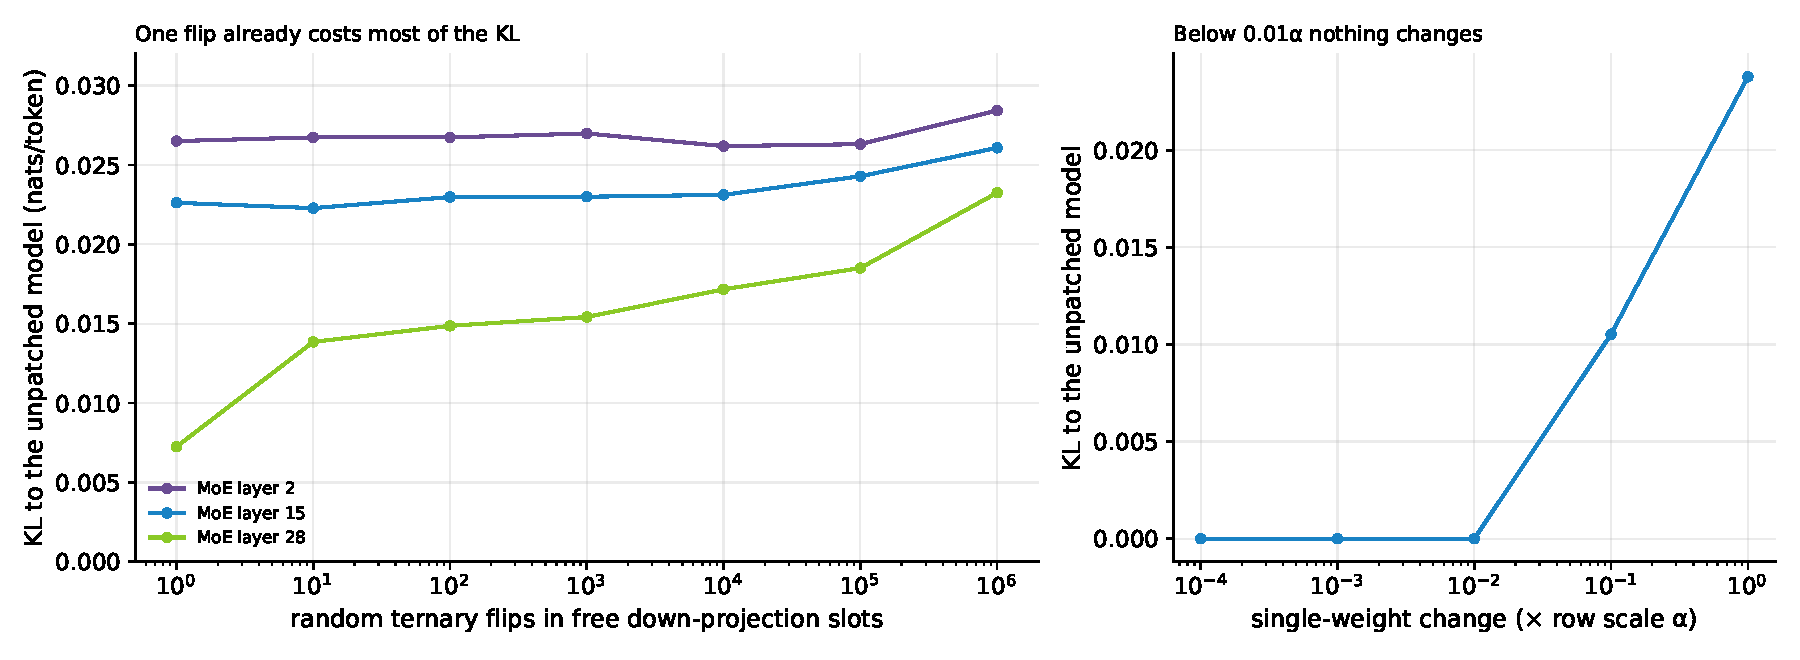
\includegraphics[width=0.90\textwidth,trim=0 26 0 0,clip]{../figures/fig_chaos_floor.pdf}
\caption{KL against the number of random ternary flips in free down-projection slots at layers 2,
15, and 28 (left), and against a single-weight change relative to its row scale (right). NLL remains within $\pm0.005$ of base for the random flips.}
\label{fig:chaos}
\end{figure}

For always-on edits the typical KL floor is about 0.02--0.027, with layer-dependent exceptions in
Table~\ref{tab:chaos}. A KL penalty mostly fights this floor: increasing its weight from 1 to 30 left
KL near 0.06 while recall fell from 48\% to 20\%. We therefore measure damage with paired $\Delta$NLL,
interpret KL relative to this floor, and use a local output penalty for preservation (\S\ref{sec:writers}).

\subsection{Recall, damage, and storage}
\begin{table}[t]\centering\small
\setlength{\tabcolsep}{3pt}
\resizebox{\textwidth}{!}{%
\begin{tabular}{lrrr}\toprule
Method & Test recall & $\Delta$NLL $\pm$ SE & Nonzero entries\\\midrule
Ternary Bop, $\tau=0.7$ & 100\% (80/80) & $+0.0266\pm0.0035$ & 812,420\\
Ternary Bop, $\tau=0.9$ & 100\% (80/80) & $+0.0314\pm0.0033$ & 588,673\\
Ternary learn-then-prune, decay 0.3 & 91.25\% (73/80) & $+0.0250\pm0.0032$ & 542,205\\
Ternary learn-then-prune, decay 0.1 & 93.75\% (75/80) & $+0.0667\pm0.0035$ & 1,857,504\\
Ternary + block scales (16), decay 0.3 & 87.5\% (70/80) & $+0.0282\pm0.0031$ & 1,125,769\\
Fp4 + local penalty $\lambda=10$, decay 0.1 & 96.25\% (77/80) & $+0.0050\pm0.0015$ & 21,265,606\\
LoRA $r=16$ + local penalty $\lambda=100$ & 97.5\% (78/80) & $+0.0005\pm0.0018$ & 22,020,096\\
LoRA $r=16$, unregularized & 97.5\% (78/80) & $+0.936\pm0.030$ & 22,020,096\\\bottomrule
\end{tabular}}

\caption{Single-seed final checkpoints: 40 facts, layers 14--15, all experts, up and down, answer-only
loss, 12 formats. Every run revokes bit-exactly by switching the patch or adapter off and comparing
logits to the unpatched model. FSA counts slots; LoRA counts fp32 parameters as trained.}
\label{tab:real}
\end{table}
Validation-selected checkpoints do not change the conclusions: Bop $\tau=0.7$ at step 250 gives
100\%/$+0.0268$, learn-then-prune at 250 gives 90\%/$+0.0282$, and regularized LoRA at 150 gives
95\%/$+0.0029$ on the test recall/damage measures.

Bop's 80/80 against LoRA's 78/80 matches, perhaps slightly exceeds, recall: two items on one seed do
not establish a significant win. LoRA with the local penalty has damage indistinguishable from zero
($+0.0005\pm0.0018$); Bop costs about $+0.027$ nats/token (about 2.7\% perplexity), roughly 50 times
LoRA's point estimate, although that estimate is near zero. Fp4 is closest to LoRA on both axes
(96.25\%, $+0.005$), but leaves the ternary format and uses a much larger patch. Unregularized LoRA
is far more damaging ($+0.94$) than any FSA run. Plain ternary writers achieve their moderate damage
without a penalty term; the ternary magnitude pin bounds how far a slot can move.

\begin{figure}[t]\centering
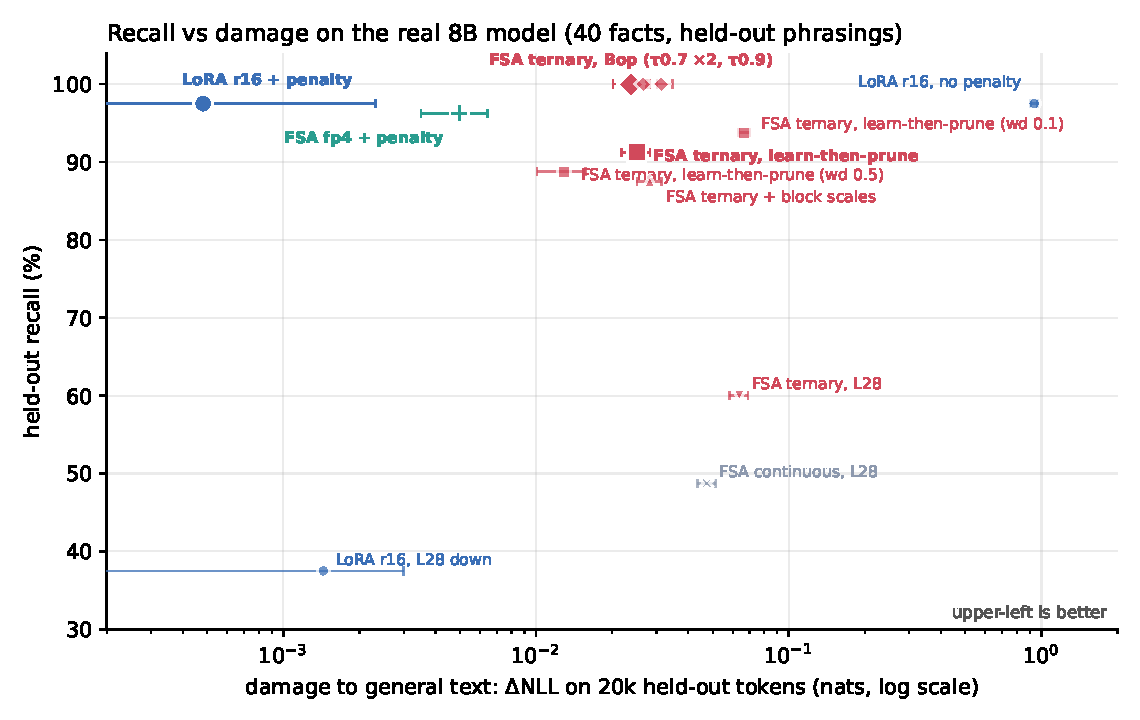
\includegraphics[width=0.85\textwidth]{../figures/fig_e2e_frontier.pdf}
\caption{Held-out recall against general-text $\Delta$NLL (log horizontal axis, SE bars).
Besides Table~\ref{tab:real}, late-layer arms use layer 28, down only, with a 2M-slot budget:
gain-minus-cost ternary selection gives 60\%/$+0.064$, continuous bf16 slots 48.75\%/$+0.047$,
and same-placement regularized LoRA 37.5\%/$+0.0014$. All are single-seed.}
\label{fig:frontier}
\end{figure}

\begin{table}[t]\centering\small
\begin{tabular}{lrr}\toprule
Patch & Entropy-coded positions + values & Indexed positions + values\\\midrule
Bop $\tau=0.7$, 812,420 slots & 0.9 MB & 2.7 MB\\
Bop $\tau=0.9$, 588,673 slots & 0.7 MB & 2.0 MB\\
Learn-then-prune, 542,205 slots & 0.6 MB & 1.8 MB\\
Fp4 + penalty, 21.3M slots & 18 MB & 80 MB\\
Block-scale run, 1,125,769 slots & 1.2 MB + block scales & 3.8 MB + block scales\\\bottomrule
\end{tabular}
\caption{Position-inclusive storage estimates. Ternary indexed storage uses a 26-bit index per slot
plus its sign. Block scales (one per 16 slots) add about 113 MB in fp32 as implemented, larger than
the adapter. LoRA has 22,020,096 parameters: 44 MB in bf16, 88 MB in fp32 as trained.}
\label{tab:storage}
\end{table}
\begin{figure}[t]\centering
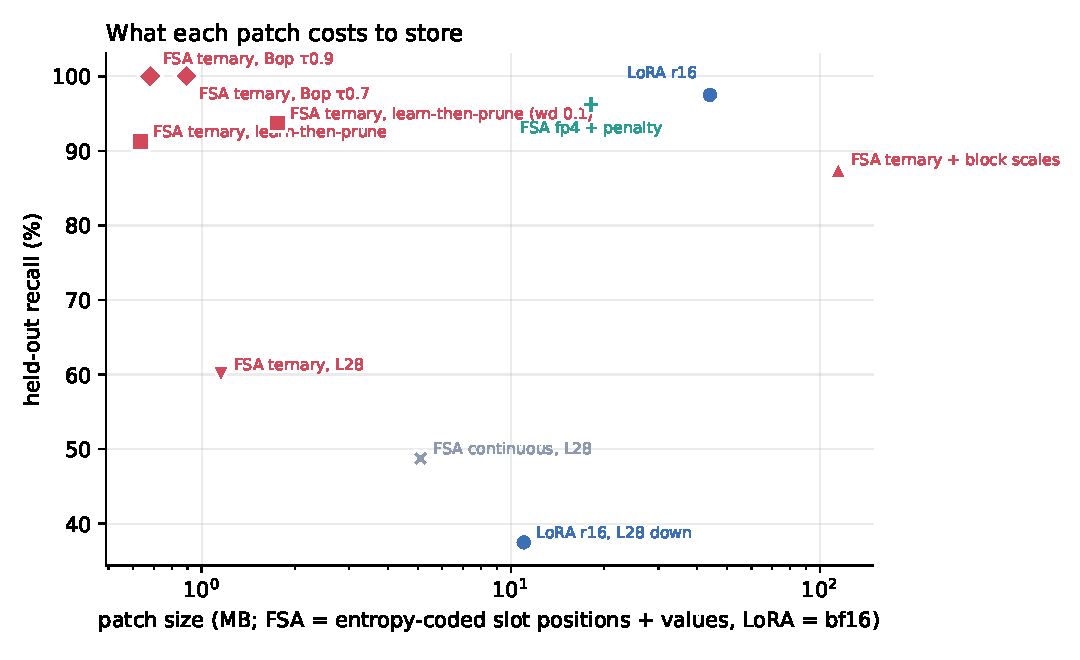
\includegraphics[width=0.85\textwidth]{../figures/fig_e2e_storage.pdf}
\caption{Recall against patch size: FSA counts entropy-coded positions and values; LoRA counts bf16
parameters. The plot excludes the block-scale run's learned scales, which as implemented exceed the
adapter's size.}
\label{fig:storage}
\end{figure}

Plain ternary patches are about 15--50 times smaller than the 44 MB bf16 adapter, depending on position
coding (Table~\ref{tab:storage}); fp4 at 18--80 MB is not a small patch. Merged ternary FSA adds no
parameters, tensors, or compute, retaining legal packed values; revocation requires the diff or original
pack. Unmerged LoRA adds a low-rank matrix multiplication per patched expert; merged LoRA requires
dense bf16 expert weights and forfeits the ternary packed format. On this fact task, regularized LoRA
remains the lower-damage method; ternary FSA trades measurable damage for matching recall, a smaller
patch, unchanged inference structure, and exact revoke. Multi-session concepts remain untested.

On isolated decoded experts with a synthetic random-fact probe, the ternary reserve learned about
500 facts per expert at about 100\% accuracy and revoked bit-exactly, but realized only 0.03--0.07
knowledge bits per slot versus 1.1--1.4 for float slots. Its 8--20 times lower weight-level output
interference than LoRA at matched knowledge did not carry over to end-to-end general-text damage:
on the full model, LoRA with a penalty is better.

\subsection{Writers}
\label{sec:writers}
\textbf{Bop, latent-free ternary.} Extending \citet{bop} from binary to ternary, each free slot holds
$q_j\in\{-1,0,+1\}$ directly, with no latent real weight. For loss gradient $g_j$, maintain
\[
m_j\leftarrow(1-\gamma)m_j+\gamma g_j,\qquad \gamma=0.05.
\]
If $q_j=0$ and $|m_j|>\tau$, birth sets $q_j\leftarrow-\operatorname{sign}(m_j)$.
If $q_j\ne0$, $|m_j|>\tau$, and $\operatorname{sign}(m_j)=q_j$, death sets $q_j\leftarrow0$:
the gradient says the current sign hurts. Reset $m_j$ to zero after each change. Thresholds are 0.7 or
0.9 times the RMS of the first answer-loss gradient over free slots, with no penalty or decay. The
threshold controls flips: small gradients need not become full $\pm\alpha$ steps, unlike Adam's
per-coordinate normalization, which can turn persistent small gradients into full flips. Nearly all
births occur within 50 steps (812,077 of the final 812,420 at $\tau=0.7$). Higher $\tau$ uses fewer
slots (589k) at slightly higher damage, so it is not a simple damage dial.

\textbf{Learn-then-prune.} Each free slot has an fp32 master $w_j$ in row-scale units. Forward uses
$q_j=\operatorname{sign}(w_j)\mathrm{I}(|w_j|>0.5)$; where $\mathrm{I}$ is the indicator; gradients pass straight through
\citep{ste}. AdamW \citep{adamw}, learning rate 0.02, applies decoupled weight decay 0.3 to masters.
The model learns early: at step 50 validation recall is 97.5\%, with 20.3M filled slots and validation
$\Delta$NLL $+2.2$. Decay pulls weakly supported masters under threshold: 3.2M slots at step 100,
1.1M at 150, and 0.54M at 300. Validation damage falls to about $+0.02$ and validation recall stays
100\%; test recall is separately 91.25\%. Damage was still falling; longer pruning may help (untested).

\textbf{Fp4 slots and local output penalty.} Four-bit float slots times $\alpha$ use AdamW decay 0.1
and add the general-text penalty
\[
\lambda\frac{\sum_{l,t}\|x_t\Delta W_l^T\|^2}{\sum_{l,t}\|x_tW_l^T\|^2},\qquad\lambda=10,
\]
where $l$ ranges over patched linear projections, $t$ over general-text tokens, $x_t$ is the input to
that projection, $W_l$ is its frozen base weight, and $\Delta W_l$ is the patch. This smooth local
penalty measures direct output change relative to base output energy without looking beyond the
patched linear, so downstream routing chaos cannot reach it. The best LoRA run uses the same penalty
with $\lambda=100$. For ternary slots it is ineffective: gradient is zero at zero, yet one birth costs a
full $\alpha^2\mathbb{E}[x^2]$; at the strength LoRA needs, it stops ternary learning entirely.

\begin{figure}[t]\centering
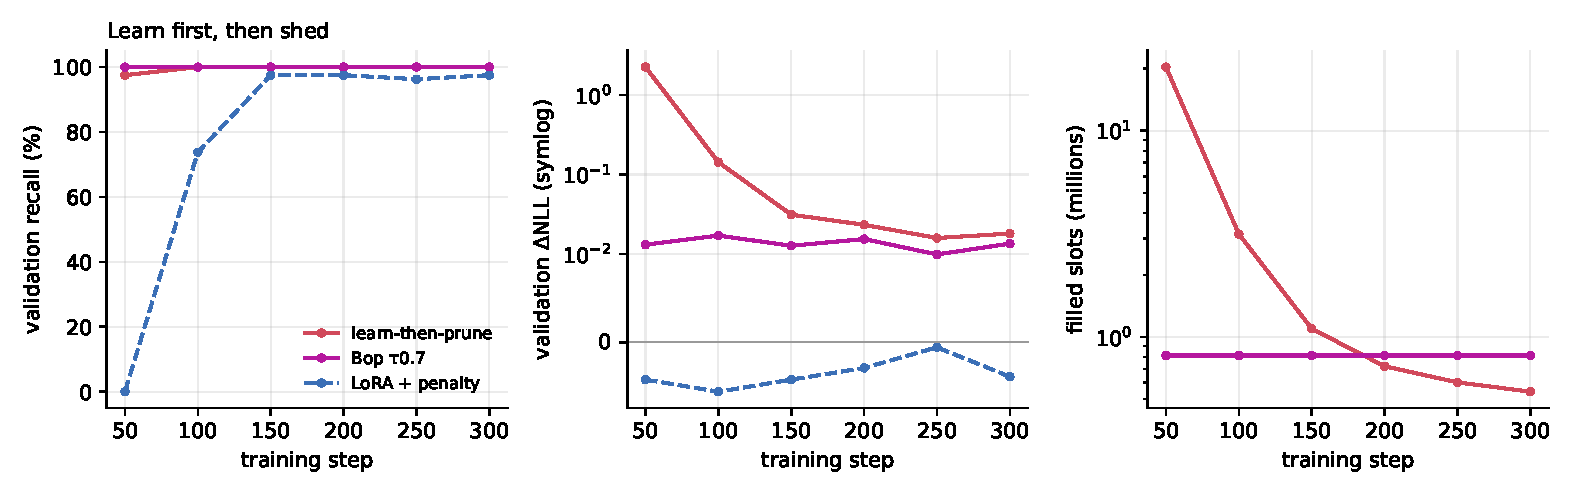
\includegraphics[width=0.90\textwidth]{../figures/fig_e2e_trajectory.pdf}
\caption{Validation recall, validation $\Delta$NLL (symmetric log scale), and filled slots (millions,
log scale) across training for learn-then-prune, Bop $\tau=0.7$, and regularized LoRA.
Validation trajectories differ from the held-out test endpoints in Table~\ref{tab:real}.}
\label{fig:trajectory}
\end{figure}

\textbf{Ingredients that mattered.} Answer-only loss avoids learning template boilerplate, which
caused most early damage with whole-sentence loss. Twelve diverse formats, including Q/A, closed the
validation-to-test gap for both FSA and LoRA (an earlier protocol reached only 54\%/56\% held-out
recall). The broad footprint mattered: 32 selected experts in one layer, down only, with 500k slots
starved capacity (19--29\% recall). Damage uses a large held-out pool, with checkpoint selection on a
separate validation pool.

\textbf{What did not work.} KL penalties fight the chaos floor and cost recall. Ternary slots with
smooth penalty and decay peak in recall, then are pruned away. Tiny fp4 values below bf16 resolution
at the base scale never learn (0\%). Patch-only learned block scales are no better than plain ternary
(87.5\%/$+0.028$) and add substantial storage. Single-late-layer continuous bf16 slots give
48.75\%/$+0.047$, versus same-placement LoRA's 37.5\%/$+0.0014$: a recall--damage trade, not an
overall improvement over LoRA. Gain-minus-cost ternary slot selection there gives 60\%/$+0.064$.

\endgroup

\section{A proposed direction (untested): multi-session personal learning}
\label{sec:direction}
The ternary reserve now carries facts on a real model (\S\ref{sec:real}). A revocable domain patch
is therefore demonstrated for this task: enable the slice for its domain; disable it to recover the base.
The personal-model application remains an untested proposal, with a narrower contract:

\begin{quote}\small
\textbf{Patch-revocation contract.} Deleting an isolated patch exactly removes \emph{that patch's parameter
contribution}. Equivalence to a model trained without its data additionally requires that no retained patch
or training state depended on it. It does not delete individual facts (facts within a slice are
superimposed), and it does not make information already in the base inaccessible.
\end{quote}

Retrieval deletes individual records while leaving the base unchanged \citep{rag,knnlm}; disabling a
per-user adapter removes that user's contribution \citep{oppu}. The case for weights is skills, style,
and policy that benefit from adaptation in every forward pass. Arbitrary facts remain a retrieval
baseline's natural task. The synthetic fp32 assay favors tuned LoRA on storage; the real ternary fact
experiment offers smaller patches at greater damage, not a general personalization result.

The pre-registered EP-1 experiment is in progress and explicitly \textbf{untested}: five sessions with
a synthetic user containing 40 policies, recurrent facts, and one-off ``lure'' facts, consolidating
self-study into free ternary slots. Success criteria fixed in advance are concept gain of at least
10 percentage points over the unpatched model on held-out probes, lure recall no more than 5 points
above it, mean general-text $\Delta$NLL at most $+0.01$ nats, retention across sessions, and exact revoke.
The comparator is regularized LoRA at the same placement; thresholds for ``match'' and ``beat'' LoRA
were fixed before the run. One seed is a pilot. Neither multi-session concept learning nor on-device
training is established: optimizer state can be large even when a final patch is small. A broader
evaluation should include local retrieval and per-user adapters on personalization benchmarks
\citep{lamp}, with unlearning measured \citep{sisa,tofu}.

\section{Limitations and the remaining experiments}
\label{sec:limits}
\textbf{Gate~0 is partly answered.} The real ternary reserve, trained through legal format values on
a real model with frozen occupancy and scales, carries the facts and has a position-inclusive storage
advantage (\S\ref{sec:real}). This does not settle damage: Bop's $+0.027$ nats exceeds the EP-1
$+0.01$ target, and regularized LoRA is better. Nor does it settle the multi-session concept task.
The decisive next evidence is that pre-registered experiment and whether ternary writers can lower
damage without losing recall. Longer pruning and packed-kernel serving remain untested.

All numbers are single-seed; the 40-fact test has only 80 items, its Q/A form resembles training,
and the roughly 20k-token damage pool cannot establish broad behavioral safety. The synthetic fp32
comparison is uncontrolled, while real-model writer and regularization choices also differ. The
chaos-floor explanation is a hypothesis. $K$ measures log-loss improvement, not semantic knowledge;
knowledge efficiency is assay- and load-specific, and from-scratch quantization results cannot predict
frozen-reserve capacity. The frozen base can augment or suppress through new paths but cannot refine
its existing weights. Exact patch-off restoration does not imply preservation while a patch is on,
per-fact deletion, or removal of knowledge already in the base.

\section{Conclusion}
The synthetic fp32 study establishes a freezing mechanism with exact masked retention, bounded
memorization, and a degrading always-on variant; its tuned LoRA comparison remains unfavorable to FSA.
On a real 8B ternary MoE, Bop recalls 80/80 held-out items from a 0.9 MB position-inclusive patch,
with exact revoke and preserved packed values, at about $+0.027$ nats/token damage. Regularized LoRA
recalls 78/80 with no measurable damage: matching recall and smaller storage do not establish an
overall FSA win. Damage is the open problem. The pre-registered multi-session concept experiment is
in progress; a private model that learns across sessions remains an untested proposal.

\small
\bibliographystyle{plainnat}
\bibliography{refs}
\end{document}
